\chapter{Радно окружење}
\label{chap:Radno okruzenje}

Један од водећих принципа у процесу развоја софтеврских решења јесте тежња да се програмски код подели у што више независних функционалних целина, које се касније на разне начине могу интегрисати. На овај начин креира се скуп библиотека које је могуће поново користити. Такође, овакав приступ олакшава развој и одржавање самог софтвера. Пре него што започне имплементацију неког софтверског решења програмер се суочава са низом избора које мора да направи:
\begin{itemize}
	\item {избор програмског језика - програм се обично реализује у једном програмском језику, бар на нивоу једне библиотеке},
	\item {избор технологије у којој ће бити имплементиран кориснички интерфејс},
	\item {избор платформе на којој ће се радити равој итд.} 
\end{itemize}

Као што је већ поменуто у секцији \textit{Преглед коришћених технологиија} \textit{OwnCloud календар конектор} је десктоп апликација, писанa у програмском језику \textit{C sharp}, развијана на \textit{XWT} платформи, и у делу који се односи на рад са календаром користи готове компоненте \textit{DDay.iCal} и \textit{CalDAV}.

\section {XWT платформа}

\textit{XWT} је \textit{.NET} мултиплатформски алат са "отвореном" лиценцом за развој апликација које могу да раде на различитим платформама, а да у основи користе заједнички код. Користи се најчешће за развој десктоп апликација које на овај начин раде на свим подржаним платформама, без потребе да се код прилагођава специфичностима сваке од њих. Разлика у односу на традиционалини приступ у развоју десктоп апликација је у томе што се контроле исцртавају динамички, у самом коду, а сам \textit{XWT API} има способност да у зависности од платформе изабере одговарајуће контроле. У наставку је дат пример кода где је приказано на који начин је креирана форма за пријаву на апликацију (Слика \ref{fig:xwt_login_form}), коришћењем \textit{XWT} алата:
\lstinputlisting[language=csharp,caption=Исцртавање форме за пријаву коришћењем \textit{XWT} алата]{primeri_koda/xwt_logIn.cs}

\begin{figure}[H]
	\centering
	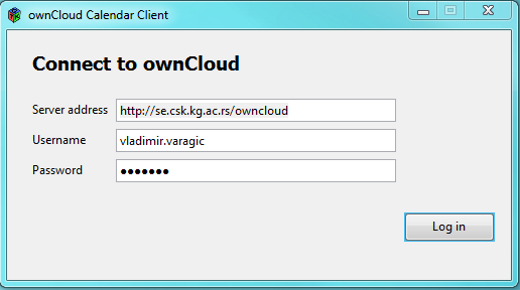
\includegraphics[scale=0.5]{slike/logInForm.png}
	\caption{Форма за пријаву на систем}
	\label{fig:xwt_login_form}
\end{figure}

\section {WebDAV}

\textit{WebDAV} представља проширење постојећег \textit{HTTP} протокола. \textit{WebDAV} протокол обезбеђује окружење које корисницима пружа могућност креирања, ажурирања, преузимања документа са удаљеног сервера. Значајно унапређење које је \textit{WebDAV} протокол донео огледа се у количини података који могу да се преносе путем мреже. Раније је број датотека био ограничен на једну датотеку по упиту, а овим протоколом се омогућава преношење више датотека. Битно својство овог протокола је и то да нуди и контролу верзије података (нпр. одржавање информација о аутору документа, датуму и времену измене документа итд.).

За разлику од других протокола за пренос података (\textit{FTP}, \textit{SSH}) за које је потребно додатно отварање портова, \textit{WebDAV} протокол користи стандардан \textit{HTTP}-порт (обично 80), па додатне конфигурације на нивоу мреже нису потребне.

Што се тиче техничке позадине \textit{WebDAV} протокола, он се састоји из скупа нових метода и заглавља постојећег \textit{HTTP} протокола и највероватније је први протокол који користи \textit{XML} језик. Методе које користи су:
\begin{itemize}
	\item {\textit{PROPFIND} -  користи се за читање особина ресурса као и евентуалне структуре истих},
	\item {\textit{PROPPATCH} - мења и брише више особина ресурса у једном кораку},
	\item {\textit{MKCOL} - креира нову колекцију},
	\item {\textit{COPY} - копира ресурс са једне на другу адресу (URI)},
	\item {\textit{MOVE} - пребацује ресурс са једне на другу адресу (URI)},
	\item {\textit{LOCK} - штити ("закључава") ресурс},
	\item {\textit{UNLOCK} - уклања заштиту ресурса}.
\end{itemize}

Готово сви оперативни ситеми имају уграђену подршку за \textit{WebDAV} протокол. У следећем примеру приказано је како се помоћу \textit{WebDAV} протокола, коришћењем \textit{PROPFIND} методе преузмa вредност поља \textit{displayName} из документа \textit{test.eml}:
\lstinputlisting[language=csharp,caption=Пример коришћења \textit{PROPFIND} методе \textit{WebDAV} протокола]{primeri_koda/webDAV_example.cs}

\section {CalDAV}

\textit{CalDAV} протокол је проширење \textit{WebDAV} протокола и представља  интернет стандард који омогућава клијенту да приступи информацијама о планираним догађајима на удаљеном серверу. Користи \textit{ICalendar}\cite{ical} формат података. Дозвољава истовремени приступ истим подацима од стране више клијената, чиме се омогућава кооперативно планирање и дељење информација. Дакле, \textit{CalDAV} je клијент/сервер протокол за календар и планирње који омогућава корисницима приступ до календара на серверу и могућност планирања догађаја са другим корисницима сервера. У наставку је дат приказ кода за преузимање информација о догађајима са \textit{OwnCloud} календара, коришћењем \textit{CalDAV} протокола:
\lstinputlisting[language=csharp,caption=Преузимање информација о догађајима са \textit{OwnCloud} календара]{primeri_koda/caldav_get_events.cs}